\documentclass{beamer}
\usepackage[utf8]{inputenc}
\usepackage{tikz}
\usepackage[framemethod=tikz]{mdframed}

\usetikzlibrary{positioning,shapes,fit,arrows}
\graphicspath{ {./images/} }

\usepackage{xcolor}
\definecolor{maroon}{cmyk}{0, 0.87, 0.68, 0.32}
\definecolor{halfgray}{gray}{0.55}
\definecolor{ipython_frame}{RGB}{207, 207, 207}
\definecolor{ipython_bg}{RGB}{247, 247, 247}
\definecolor{ipython_red}{RGB}{186, 33, 33}
\definecolor{ipython_green}{RGB}{0, 128, 0}
\definecolor{ipython_cyan}{RGB}{64, 128, 128}
\definecolor{ipython_purple}{RGB}{170, 34, 255}

\usepackage{listings}
\lstset{
    breaklines=true,
    %
    extendedchars=true,
    literate=
    {á}{{\'a}}1 {é}{{\'e}}1 {í}{{\'i}}1 {ó}{{\'o}}1 {ú}{{\'u}}1
    {Á}{{\'A}}1 {É}{{\'E}}1 {Í}{{\'I}}1 {Ó}{{\'O}}1 {Ú}{{\'U}}1
    {à}{{\`a}}1 {è}{{\`e}}1 {ì}{{\`i}}1 {ò}{{\`o}}1 {ù}{{\`u}}1
    {À}{{\`A}}1 {È}{{\'E}}1 {Ì}{{\`I}}1 {Ò}{{\`O}}1 {Ù}{{\`U}}1
    {ä}{{\"a}}1 {ë}{{\"e}}1 {ï}{{\"i}}1 {ö}{{\"o}}1 {ü}{{\"u}}1
    {Ä}{{\"A}}1 {Ë}{{\"E}}1 {Ï}{{\"I}}1 {Ö}{{\"O}}1 {Ü}{{\"U}}1
    {â}{{\^a}}1 {ê}{{\^e}}1 {î}{{\^i}}1 {ô}{{\^o}}1 {û}{{\^u}}1
    {Â}{{\^A}}1 {Ê}{{\^E}}1 {Î}{{\^I}}1 {Ô}{{\^O}}1 {Û}{{\^U}}1
    {œ}{{\oe}}1 {Œ}{{\OE}}1 {æ}{{\ae}}1 {Æ}{{\AE}}1 {ß}{{\ss}}1
    {ç}{{\c c}}1 {Ç}{{\c C}}1 {ø}{{\o}}1 {å}{{\r a}}1 {Å}{{\r A}}1
    {€}{{\EUR}}1 {£}{{\pounds}}1
}

\usepackage{animate}

%%
%% Python definition (c) 1998 Michael Weber
%% Additional definitions (2013) Alexis Dimitriadis
%% modified by me (should not have empty lines)
%%
\lstdefinelanguage{iPython}{
    morekeywords={access,and,break,class,continue,def,del,elif,else,except,exec,finally,for,from,global,if,import,in,is,lambda,not,or,pass,print,raise,return,try,while},%
    %
    % Built-ins
    morekeywords=[2]{abs,all,any,basestring,bin,bool,bytearray,callable,chr,classmethod,cmp,compile,complex,delattr,dict,dir,divmod,enumerate,eval,execfile,file,filter,float,format,frozenset,getattr,globals,hasattr,hash,help,hex,id,input,int,isinstance,issubclass,iter,len,list,locals,long,map,max,memoryview,min,next,object,oct,open,ord,pow,property,range,raw_input,reduce,reload,repr,reversed,round,set,setattr,slice,sorted,staticmethod,str,sum,super,tuple,type,unichr,unicode,vars,xrange,zip,apply,buffer,coerce,intern},%
    %
    sensitive=true,%
    morecomment=[l]\#,%
    morestring=[b]',%
    morestring=[b]",%
    %
    morestring=[s]{'''}{'''},% used for documentation text (mulitiline strings)
    morestring=[s]{"""}{"""},% added by Philipp Matthias Hahn
    %
    morestring=[s]{r'}{'},% `raw' strings
    morestring=[s]{r"}{"},%
    morestring=[s]{r'''}{'''},%
    morestring=[s]{r"""}{"""},%
    morestring=[s]{u'}{'},% unicode strings
    morestring=[s]{u"}{"},%
    morestring=[s]{u'''}{'''},%
    morestring=[s]{u"""}{"""},%
    %
    % {replace}{replacement}{lenght of replace}
    % *{-}{-}{1} will not replace in comments and so on
    literate=
    {á}{{\'a}}1 {é}{{\'e}}1 {í}{{\'i}}1 {ó}{{\'o}}1 {ú}{{\'u}}1
    {Á}{{\'A}}1 {É}{{\'E}}1 {Í}{{\'I}}1 {Ó}{{\'O}}1 {Ú}{{\'U}}1
    {à}{{\`a}}1 {è}{{\`e}}1 {ì}{{\`i}}1 {ò}{{\`o}}1 {ù}{{\`u}}1
    {À}{{\`A}}1 {È}{{\'E}}1 {Ì}{{\`I}}1 {Ò}{{\`O}}1 {Ù}{{\`U}}1
    {ä}{{\"a}}1 {ë}{{\"e}}1 {ï}{{\"i}}1 {ö}{{\"o}}1 {ü}{{\"u}}1
    {Ä}{{\"A}}1 {Ë}{{\"E}}1 {Ï}{{\"I}}1 {Ö}{{\"O}}1 {Ü}{{\"U}}1
    {â}{{\^a}}1 {ê}{{\^e}}1 {î}{{\^i}}1 {ô}{{\^o}}1 {û}{{\^u}}1
    {Â}{{\^A}}1 {Ê}{{\^E}}1 {Î}{{\^I}}1 {Ô}{{\^O}}1 {Û}{{\^U}}1
    {œ}{{\oe}}1 {Œ}{{\OE}}1 {æ}{{\ae}}1 {Æ}{{\AE}}1 {ß}{{\ss}}1
    {ç}{{\c c}}1 {Ç}{{\c C}}1 {ø}{{\o}}1 {å}{{\r a}}1 {Å}{{\r A}}1
    {€}{{\EUR}}1 {£}{{\pounds}}1
    %
    {^}{{{\color{ipython_purple}\^{}}}}1
    {=}{{{\color{ipython_purple}=}}}1
    %
    {+}{{{\color{ipython_purple}+}}}1
    {*}{{{\color{ipython_purple}$^\ast$}}}1
    {/}{{{\color{ipython_purple}/}}}1
    %
    {+=}{{{+=}}}1
    {-=}{{{-=}}}1
    {*=}{{{$^\ast$=}}}1
    {/=}{{{/=}}}1,
    literate=
    *{-}{{{\color{ipython_purple}-}}}1
     {?}{{{\color{ipython_purple}?}}}1,
    %
    identifierstyle=\color{black}\ttfamily,
    commentstyle=\color{ipython_cyan}\ttfamily,
    stringstyle=\color{ipython_red}\ttfamily,
    keepspaces=true,
    showspaces=false,
    showstringspaces=false,
    %
    rulecolor=\color{ipython_frame},
    frame=single,
    frameround={t}{t}{t}{t},
    framexleftmargin=6mm,
    numbers=left,
    numberstyle=\tiny\color{halfgray},
    %
    %
    backgroundcolor=\color{ipython_bg},
    %   extendedchars=true,
    basicstyle=\scriptsize,
    keywordstyle=\color{ipython_green}\ttfamily,
}

% \definecolor{light-gray}{gray}{0.95}
\surroundwithmdframed[
  hidealllines=true,
  innerleftmargin=15pt,
  innertopmargin=0pt,
  innerbottommargin=0pt]{lstlisting}

\usetheme{Berlin}
\usefonttheme[onlymath]{serif}

\usepackage{censor}

% \usecolortheme{crane}
\setbeamertemplate{navigation symbols}{}%remove navigation symbols

\title{Procedural Music Generation}
\subtitle{Generating (\censor{shitty} MIDI) music in Python}
% \author{Shon Verch}
\institute{Stephen Lewis Secondary School}
\author{Computer Science Club}
\date{May 24, 2019}

\setbeamertemplate{frametitle continuation}[from second][(contd.)]

\newcommand{\sectionFrame}[3]
{
    \section{#3}
    \begin{frame}
    \begin{block}{}
    \begin{center}
        \Huge{#1}\\[0.5ex]
        \large{#2}
    \end{center}
    \end{block}
    \end{frame}
}

\usepackage{caption}

\begin{document}
\begin{frame} 
\titlepage 
\end{frame}

\section{Introduction}
\subsection{Overview}
\begin{frame}{Premise}
\only<1-3>{\par{\LARGE{I have always wanted to compose music.}}\\~\ }
\only<2-3>{\par{\textit{However,} I have no musical talents---or any for that matter.}\\~\ }
\only<3>{\par{Fortunately, we can \textbf{generate} music without having any musical talents!}}
\end{frame}

\begin{frame}{Objective}
In this lesson, we will be learning how we can apply a few patterns and some simple rules to procedurally generate music.\\~\

We will be using:
\begin{enumerate}
    \item Python
    \item A fair bit of maths
    \item Our creative ``intuition''
\end{enumerate}
\end{frame}

\subsection{MIDI}
\begin{frame}[t]{Introduction to MIDI}
\begin{block}{Definition}
MIDI (or Musical Instrument Digital Interface) is simply a protocol for communication between digital musical instruments and the computer.
\end{block}

The beauty of MIDI is that
\begin{enumerate}[(a)]
    \item it is lightweight
    \item consists of events/instructions that we can \textit{create and manipulate}
\end{enumerate}
\end{frame}

\begin{frame}{The MIDI Note System}
MIDI uses positive integers to represent notes:
\begin{itemize}
    \item $60$ represents the middle C
    \item Adding or subtracting $1$ goes up or down a semitone respectively
    \item Adding or subtracting $12$ increases or decreases the note by a single octave respectively
\end{itemize}
There are $128$ notes from $0$ to $127$.
\end{frame}

\begin{frame}[allowframebreaks]{What does this mean for us?}
We can use any function, $f$, to generate notes based on some parameter(s) so long as:
\begin{equation*}
    f:X \to \mathbb{N}_{< 128}^{0},
\end{equation*}
where $X$ denotes some arbitrary space.

\framebreak
Suppose that we want to play the notes, in succession, from the middle C, we can use a simple linear function to model this series of notes: 
$$f(x)=60+x,\hspace{1em}\text{where\;\;}0\leq x\leq 68,$$
which will generate the equivalent MIDI note for a value of $x$. In this case, $f:\mathbb{N}^{0}_{\leq 68}\to\mathbb{N}_{<128}^{0}$, which satisfies our restriction on the codomain of a `note function.'
\end{frame}

\begin{frame}[allowframebreaks,fragile]{MIDI manipulation in Python}
\texttt{MIDIUtil} is a Python library that allows us to write MIDI files.
\begin{center}
\begin{lstlisting}[language=iPython]
from midiutil import MIDIFile

midi_file = MIDIFile(1) # Create MIDI file with one track.
midi_file.addTempo(0, 0, 120) # set the tempo to 120 BPM on track 0, at time 0.
for i in range(10):
    # midi_file.addNote(track, channel, note, time, duration, volume)
    # time is in beats (from the start of the song) and duration is in quarter notes.
    midi_file.addNote(0, 0, 60 + i, i, 1, 100)
\end{lstlisting}
\end{center}

\framebreak

Exporting MIDI files is as simple as any other file I/O in Python. The following code outputs a MIDI file called \texttt{example.mid}:
\begin{center}
\begin{lstlisting}[language=iPython]
def save_midi(midi_handle, filename):
    destination = f'{filename}.mid'
    with open(destination, 'wb') as output_file:
        midi_handle.writeFile(output_file)
        
# export MIDI
save_midi(midi_file, 'example')
\end{lstlisting}
\end{center}
\end{frame}

\begin{frame}[fragile,allowframebreaks]{Example: Fun with Multiples!}
\only<1>{
We map a note to a set of integers. Then, for each positive integer $i$, we play the assigned notes corresponding to the multiples of $i.$\\~\

For example, for the integer $10$, we play the notes assigned to $2$, $5$, and $10.$
}

\framebreak

\begin{center}
\begin{lstlisting}[language=iPython]
# ... midi_file preamble

multiples = {
    2: 60, # C4
    3: 62, # D4
    4: 65, # F4
    5: 67  # G4
}

# N is some positive integer greater than one.
for i in range(1, N + 1):
    for multiple in multiples:
        if i % multiple == 0:
            note = multiples[multiple]
            midi_file.addNote(0, 0, note, i, 1, 100)
\end{lstlisting}
\end{center}
\end{frame}

\begin{frame}[fragile,allowframebreaks]{Example: Fibonacci Numbers}
We map $0$ to D5-sharp, $1$ to E5, and so on... to some integer value $n$. Then, for each Fibonacci number, we can play the associated note for that Fibonacci number modulo $n$.\\~\

Alternatively, we map each positive integer to a note. Then, we can play the associated note for each Fibonacci number.
\framebreak
\begin{center}
\begin{lstlisting}[language=iPython]
# ... midi_file preamble
# generate note mapping
notes = {}
for i in range(10):
    # i semitones from D5-Sharp (75)
    notes[i] = 75 + i

# N is some positive integer greater than one.
for i in range(N):
    # get_fibonacci_number(n) returns the n-th fibonacci number (one-based)
    note = notes[get_fibonacci_number(i + 1) % 10]
    midi_file.addNote(0, 0, note, i, 1, 100)
\end{lstlisting}
\end{center}
\end{frame}

\subsection{Advanced MIDI}
\begin{frame}{Note duration}
Notice that the \lstinline[language=iPython]{MIDIFile.addNote} method takes in a \lstinline[language=iPython]{duration} parameter.\\~\

The duration of a note is given in quarter notes and can be any positive real number. Therefore, just as our notes, we can use any function, $g$, to generate note duration so long as:
$$g : X \to \mathbb{R}^{+},$$
where $X$ denotes some arbitrary space.
\end{frame}

\begin{frame}[fragile,allowframebreaks]{Example: Periodic Note Duration}
Let's take our previous example (``Fun with Multiples!'') and apply a sinusoidal function to its duration; however, before we can do that, we must apply a few transformations to $\sin(x)$:
\begin{enumerate}
    \item Vertical shift by $\frac{11}{20}$
    \item Vertical compression by $\frac{9}{20}$ so that the maximum is $1$ and minimum is $\frac{1}{10}.$ 
\end{enumerate}
Therefore, $\displaystyle{g(x)=\frac{9}{20}\sin(x)+\frac{11}{20}.}$
\framebreak
\begin{center}
\begin{lstlisting}[language=iPython]
# ... midi_file preamble
from math import sin

# define multiple mapping

# N is some positive integer greater than one.
time = 0
for i in range(1, N + 1):
    duration = 0.45 * sin(i) + 0.55
    for multiple in multiples:
        if i % multiple == 0:
            note = multiples[multiple]
            midi_file.addNote(0, 0, note, time, duration, 100)
    time += duration
\end{lstlisting}
\end{center}
\end{frame}

\begin{frame}[fragile,allowframebreaks]{Multiple Channels}
MIDI supports multiple channels and we can leverage that to create more interesting music. The \lstinline[language=iPython]{MIDIFile} constructor takes in a channel parameter indicating the number of channels in the MIDI file.
\begin{center}
\begin{lstlisting}[language=iPython]
from midiutil import MIDIFile

midi_file = MIDIFile(N) # Create MIDI file with N tracks.
\end{lstlisting}
\end{center}
\framebreak
Adding a note to a channel is easy: simply pass in the channel index into the \lstinline[language=iPython]{MIDIFile.addNote} method:
\begin{center}
\begin{lstlisting}[language=iPython]
from midiutil import MIDIFile

# add a note to the i-th channel
midi_file.addNote(0, i, note, time, duration, volume)
\end{lstlisting}
\end{center}
\end{frame}

\begin{frame}{A few more notes...}
Along with the properties we have already discusssed, we can manipulate
\begin{enumerate}
    \item Volume
    \item Tempo
    \item Tracks
\end{enumerate}
\end{frame}

\begin{frame}{These \textit{don't} sound good though...}
\par{\LARGE{\textbf{But}, it is clear how we can use these MIDI properties to generate music.}\\~\ }
\par{We will create rules for the tempo, duration, and notes that sound good together and we will use these rules to generate songs.}
\end{frame}
\subsection*{Conclusion}
\begin{frame}{Approaches to Generating Music}
There are a variety of techniques that we can use to generate music, some more complex than others:
\begin{enumerate}
    \item `Pattern-based' generation
    \item Markov chains (statistical models)
    \item Cellular automata
    \item Machine learning
\end{enumerate}
\end{frame}

\section{Pattern-based generation}
\begin{frame}{Introduction}
\par{We find that applying some basic patterns related to key, duration, and tempo, we can start to generate some pretty good music with relatively minimal effort.\\~\ }

\par{Of course, the rules that dictate the procedural generation are fairly subjective so by all means, play around with them and make your own!}
\end{frame}

\begin{frame}{Main Components \& Important Things to Remember}
\begin{itemize}
    \item \textbf{Rhythm}: playing notes at a specific interval
    \item \textbf{Emphasis}: To make a rhythm interesting, we emphasise the first note in every measure. We should also emphasise the beat half way through the measure (the down beat).
    \item \textbf{Repetition}
\end{itemize}
\end{frame}

\begin{frame}{Scales}
It's important to keep in mind the interval of notes: certain notes just sound better together and we can use this to our advantage.
\begin{itemize}
    \item Major: happy
    \item Harmonic Minor: creepy
    \item Natural minor: ``epic''
    \item Melodic minor, ascending: mysterious
    \item Melodic minor, descending: calm
\end{itemize}
\end{frame}

\section{Markov-chains}
\begin{frame}{Basic Definition}
\begin{columns}
\column{0.7\linewidth}
A Markov chain is a stochastic model that, based on an input, gives a set of outcomes. It describes ``a sequence of possible events in which the probability of each event depends only on the state attained in the previous event.''
\column{0.3\linewidth}
\centering
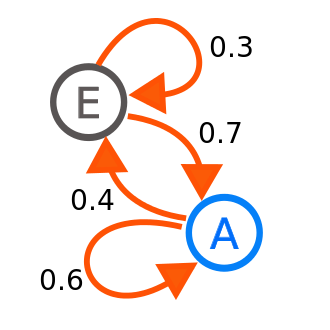
\includegraphics[width=3.5cm]{lessons/images/markov.png}
\end{columns}
\end{frame}

\begin{frame}{Applied to music}
We can use a Markov chain to determine the probability of the next note. For example, suppose our song consists of the notes $A$-$B$-$C$, our Markov chain might say that there is a $30$\% chance for an $E$, $10$\% chance for an $F$, and etc...
\end{frame}

\section{Cellular Automota}
\begin{frame}{Cellular Automota}
% \begin{columns}
% \column{0.7\linewidth}
A system consisting of a grid of cells where each cell has its own state. Then, in every progression of the system, the cells change state based on some rule.
% \column{0.3\linewidth}
%  \animategraphics[loop,controls,width=0.3\linewidth]{10}{lessons/images/cellular_automota/cgif}{0}{16}
% \end{columns}.
\end{frame}

\begin{frame}[allowframebreaks]{1D Cellular Automota}
\par{Our grid is a one-dimensional array and our cells have a binary state: on or off. The state of the $i$-th cell in the system at time $t$, $C(i,t)$ is then determined by its neighbours and the previous generation, $t-1$.\\~\ }

\par{Since there are only $8$ ($2^2$) states that our cells can be, we define them exhaustively: we define what happens for the given states of the cells at $i-1$, $i$, and $i+1$.}
\framebreak
\begin{center}
\begin{tabular}{ c|c|c||c } 
$\mathcal{S}(i-1)$ & $\mathcal{S}(i)$ & $\mathcal{S}(i+1)$ & $C(i,t)$\\
 \hline
 1 & 1 & 1 & 1 \\ 
 1 & 1 & 0 & 1 \\ 
 1 & 0 & 1 & 1 \\
 1 & 0 & 0 & 0 \\
 0 & 1 & 1 & 1 \\
 0 & 1 & 0 & 1 \\
 0 & 0 & 1 & 0 \\
 0 & 0 & 0 & 1
\end{tabular}
\end{center}
\end{frame}

\begin{frame}[t]{The rule is everything!}
\par{Based on the rule of the cellular automota system, we can get wildly different results. The following pattern emerges from starting with a single `on' cell in the middle of a row of 15 `off' cells.\\~\ }

\par{\centering{

\includegraphics[width=3.5cm]{lessons/images/1dca.png}}}
\end{frame}

\end{document}